%# -*- coding:utf-8 -*-
\subsection[冠状动脉分割II]{改进的基于CURVES的冠状动脉分割}

\begin{frame}
\begin{itemize}
  \item \textbf{改进的冠状动脉分割流程}:
\end{itemize}
\begin{figure}[t]
\centering
%# -*- coding:utf-8 -*-
\begin{tikzpicture}[scale=.37]

\draw [black,thick,rounded corners] (-3,0) rectangle (3,2);            % binary threshold
\draw [black,thick,rounded corners] (-3,3) rectangle (3,5);  % CURVES

\draw [black,thick,rounded corners] (-8,7) rectangle (-2,9);   % initial contours

\draw [black,thick,rounded corners] (2,7) rectangle (8,9);     % feature images

\draw [black,thick,rounded corners] (-3,11) rectangle (3,13);  % thresholding
\draw [black,thick,rounded corners] (-3,14) rectangle (3,16);  % curvature anisotropic diffusion
\draw [black,thick,rounded corners] (-3,17) rectangle (3,19);  % raw input

\node [above right] at (-2.25,0.25) {\scriptsize \fs \bf 二值阈值滤波};
\node [above right] at (-2.25,3.25) {\scriptsize \fs \bf 测地活动轮廓};

\node [above right] at (-7.65,7.35) {\scriptsize \fs \bf 初始水平集演进};

\node [above right] at (2.82,7.35) {\scriptsize \fs \bf 特征图像计算};

\node [above right] at (-2.3,11.35) {\scriptsize \fs \bf 二值阈值滤波};
\node [above right] at (-2.9,14.35) {\scriptsize \fs \bf 曲率各向异性扩散};
\node [above right] at (-1.95,17.35) {\scriptsize \fs \bf ROI体数据};

\draw [<-,thick] (0,2) -- (0,3);

\draw [<-,thick] (0,5) -- (0,6);
\draw [thick] (-5,6) -- (5,6);
\draw [thick] (-5,6) -- (-5,7);
\draw [thick] (5,6) -- (5,7);

\draw [<-,thick] (-5,9) -- (-5,10);
\draw [<-,thick] (5,9) -- (5,10);
\draw [thick] (-5,10) -- (5,10);
\draw [thick] (0,10) -- (0,11);

\draw [<-,thick] (0,13) -- (0,14);
\draw [<-,thick] (0,16) -- (0,17);

\end{tikzpicture} 
% 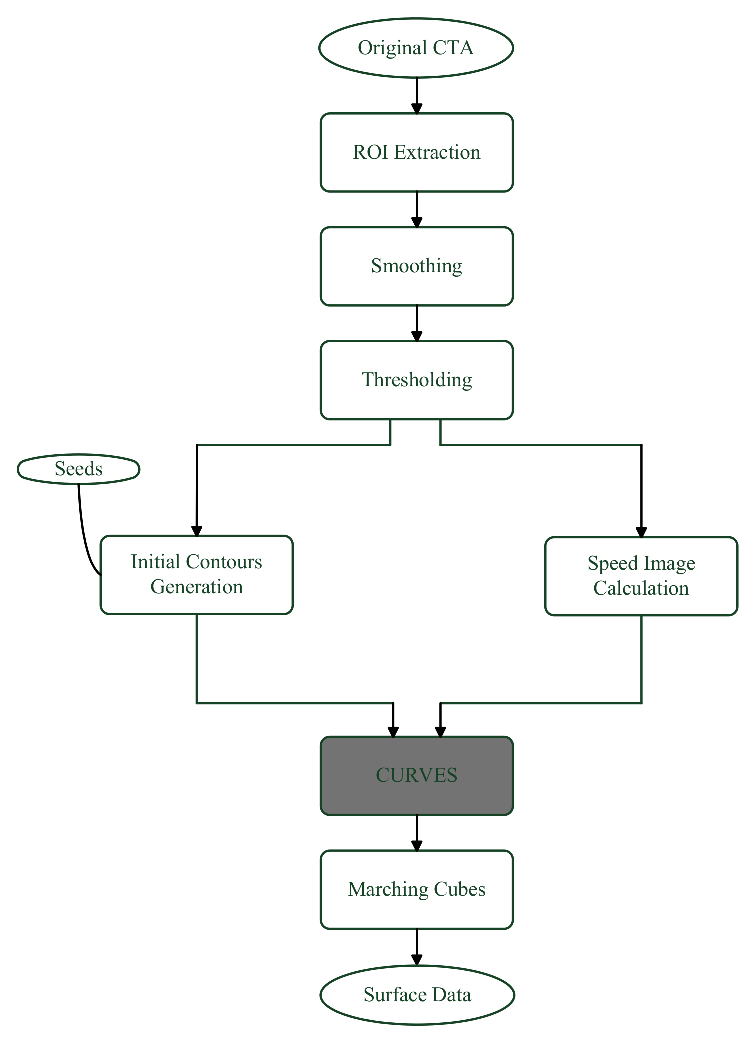
\includegraphics[width=3.2in]{Figures/coronary/DataFlow}
% \caption[心脏区域的ROI提取]{心脏区域的ROI提取。}
% \label{fig:coronary_ROI}
\end{figure}
\end{frame}

\begin{frame}
\begin{itemize}
\item \textbf{多尺度管状物增强~[Sato(1998)]}
\begin{itemize}
\pause \item \textbf{三维线滤波}:等价为三维图像$I(\cdot)$的Hessian阵的计算:
\begin{gather*}
\mathcal{H} = \nabla^2 I =
\begin{bmatrix}
I_{xx} & I_{xy} & I_{xz} \\ I_{yx} & I_{yy} & I_{yz} \\ I_{zx} & I_{zy} & I_{zz}
\end{bmatrix}
\end{gather*}
\begin{itemize}
\item \textbf{特征值}: $\lambda_1$,$\lambda_2$,和$\lambda_3$,降序排列
\item \textbf{相应的特征向量}: $e_1$,$e_2$,和$e_3$
\item $I_{xx} = \frac{\partial^2 I}{\partial^2 x}$, $I_{xy} = \frac{\partial^2 I}{\partial x \partial y}$, \dots
\end{itemize}
\pause \item \textbf{滤波响应的多尺度整合}:求各尺度响应的最大值
\end{itemize}
\end{itemize}
\end{frame}

\begin{frame}
\begin{itemize}
\item \textbf{增强不同形状所需的特征值}
\end{itemize}
\begin{table}[h]
\renewcommand{\arraystretch}{0.5}
\centering
\begin{tabular*}{80mm}{cc}
\toprule
\hspace{5mm} \bfseries \small{物体形状}  & \hspace{15mm}                    \bfseries \small{特征值}                       \\
\midrule
\hspace{5mm} \small{明亮的管状}          & \hspace{15mm}  \small{$\lambda_1 \approx 0, \lambda_2 \approx \lambda_3 \ll 0$} \\
\hspace{5mm} \small{暗淡的管状}          & \hspace{15mm}  \small{$\lambda_1 \approx 0, \lambda_2 \approx \lambda_3 \gg 0$} \\
\hspace{5mm} \small{明亮的盘状}          & \hspace{15mm}  \small{$\lambda_1 \approx \lambda_2 \approx 0, \lambda_3 \ll 0$} \\
\hspace{5mm} \small{暗淡的盘状}          & \hspace{15mm}  \small{$\lambda_1 \approx \lambda_2 \approx 0, \lambda_3 \gg 0$} \\
\hspace{5mm} \small{明亮的球状}          & \hspace{15mm}  \small{$\lambda_1 \approx \lambda_2 \approx \lambda_3 \ll 0$}    \\
\hspace{5mm} \small{暗淡的球状}          & \hspace{15mm}  \small{$\lambda_1 \approx \lambda_2 \approx \lambda_3 \gg 0$}    \\
\bottomrule
\end{tabular*}
\end{table}
\end{frame}

\begin{frame}
\begin{itemize}
\item \textbf{推广的线形相似性测度} (\alert{$\lambda_1 \approx 0$ and $\lambda_2 \approx \lambda_3 \ll 0$})
\pause \begin{equation*}
\lambda_{123} =
\begin{cases}
\left| \lambda_3 \right| \left( \frac{\lambda_2}{\lambda_3} \right)^{\gamma_{23}} \left( 1 + \frac{\lambda_1}{\left| \lambda_2 \right|} \right)^{\gamma_{12}},        & \lambda_1 \le 0 \\%
\left| \lambda_3 \right| \left( \frac{\lambda_2}{\lambda_3} \right)^{\gamma_{23}} \left( 1 - \alpha \frac{\lambda_1}{\left| \lambda_2 \right|} \right)^{\gamma_{12}}, & \frac{\left| \lambda_2 \right|}{\alpha} > \lambda_1 > 0 \\%
0,                                                                                                                                                                    & \text{其它} %
\end{cases}
\end{equation*}
% \end{itemize}
\begin{itemize}
\pause \item \textbf{附加参数}:$\gamma_{12}$,$\gamma_{23}$,和$\alpha$,全部为正
\begin{itemize}
\item $\gamma_{12} \in [0, \infty)$:辨别出分支结构与噪音以及伪分支结构
\item $\gamma_{23} \in [0, \infty)$:控制图像锐度
\item $\alpha \in (0, 1.0]$:对于任意$\lambda_1$,保持函数最后一项的对称性
\end{itemize}
\end{itemize}
\end{itemize}
\end{frame}

\begin{frame}
\begin{itemize}
  \item \textbf{心脏区域的VOI提取}:
  \begin{itemize}
  \pause \item 设定长方体区域的起点和尺寸
  \pause \item 缩小处理区域,减轻运算负担
  \end{itemize}
\end{itemize}
\begin{figure}[t]
\centering
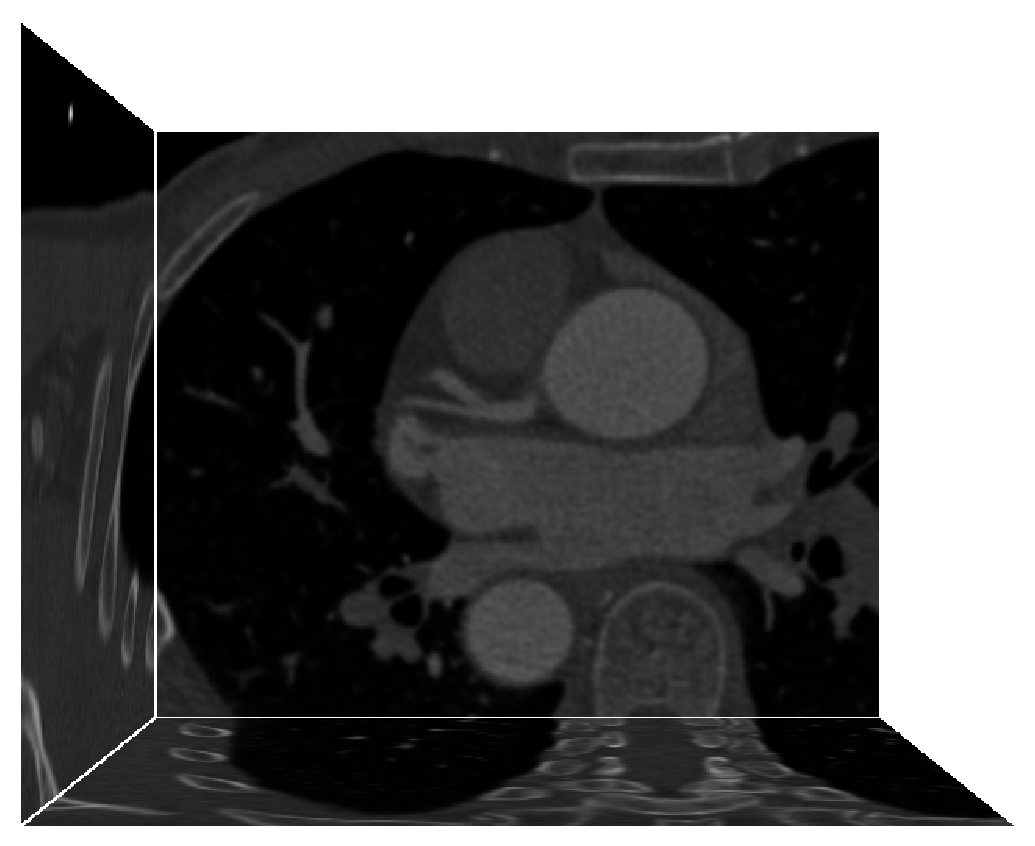
\includegraphics[width=1.5in]{../../Figures/coronary/coronary_enhanced/original}
% \caption[心脏区域的ROI提取]{心脏区域的ROI提取。}
% \label{fig:coronary_ROI}
\end{figure}
\end{frame}

\begin{frame}
\begin{itemize}
  \item \textbf{管状物体增强}:
  \begin{enumerate}
    \onslide<1-3> \item 二值阈值滤波($\text{TH}_{\text{lower}} = 300$, $\text{TH}_{\text{upper}} = 600$)
    \onslide<3> \item 管状物体增强($\sigma = 0.9$, $\gamma_{12} = 0.1$, $\gamma_{23} = 2.0$)
  \end{enumerate}
\end{itemize}
\begin{columns}[b,onlytextwidth]
\begin{column}{.5\textwidth}
\onslide<2-3> \begin{figure}[t]
\centering
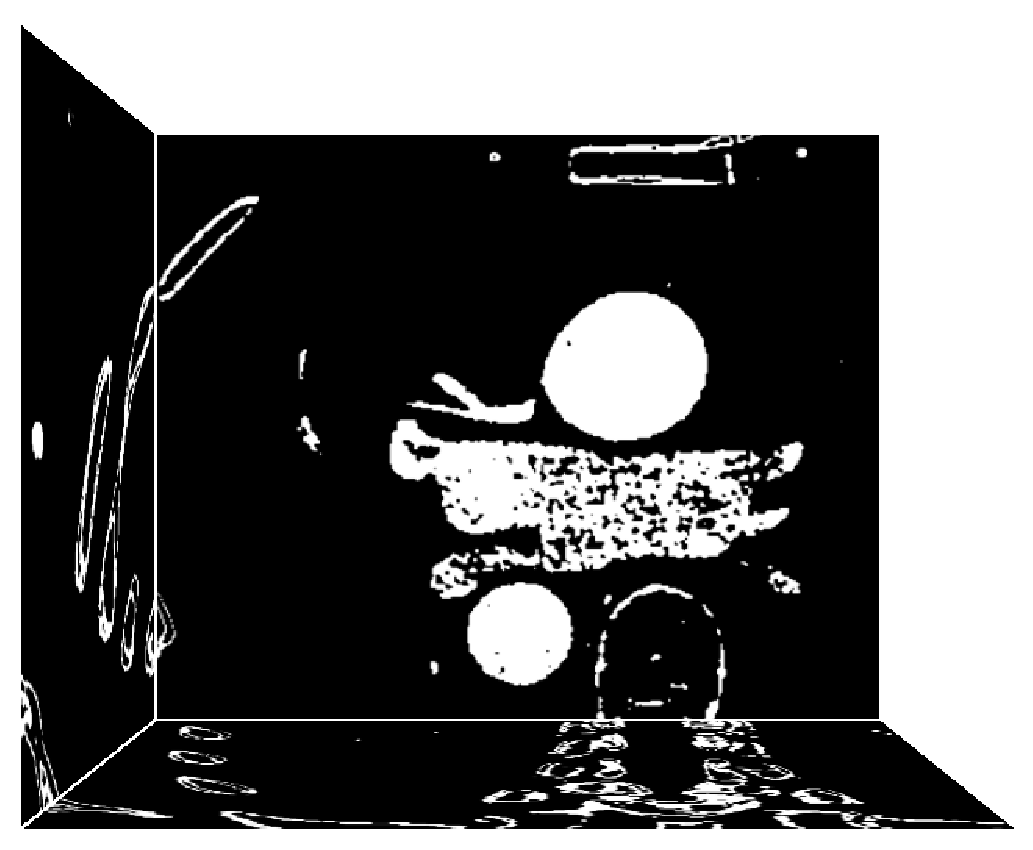
\includegraphics[height=1.5in]{../../Figures/coronary/coronary_enhanced/binary1.eps}
\end{figure}
\end{column}
\begin{column}{.5\textwidth}
\onslide<3> \begin{figure}[t]
\centering
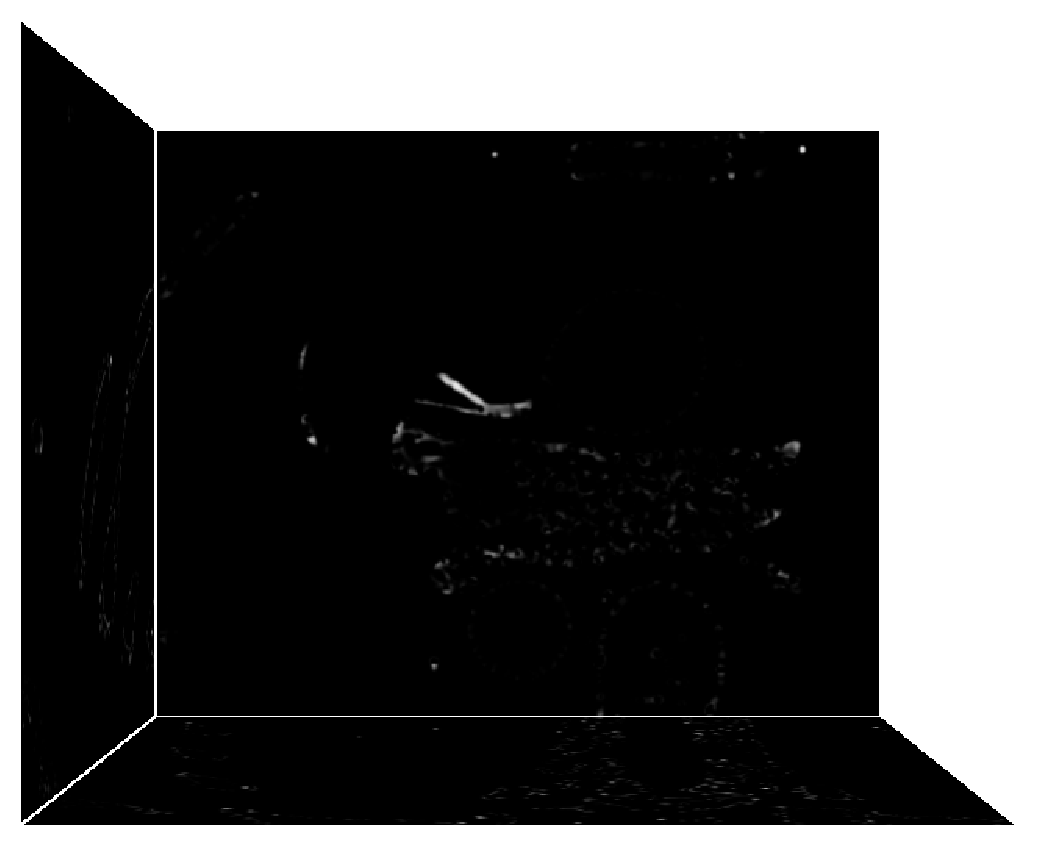
\includegraphics[height=1.5in]{../../Figures/coronary/coronary_enhanced/hessian.eps}
\end{figure}
\end{column}
\end{columns}
% \centering{\textbf{\alert 增强后的管状物亮度值过低,且不均匀}}
\end{frame}

\begin{frame}
\begin{itemize}
  \item \textbf{两种像素亮度处理结果对比}:
  \begin{enumerate}
    \onslide<1-3> \item 非线性亮度映射($m = 80$, $n = 120$)
    \onslide<3> \item 二值阈值滤波($\text{TH}_{\text{lower}} = 40$, $\text{TH}_{\text{upper}} = 200$)
  \end{enumerate}
\end{itemize}
\begin{columns}[b,onlytextwidth]
\begin{column}{.5\textwidth}
\onslide<2-3> \begin{figure}[t]
\centering
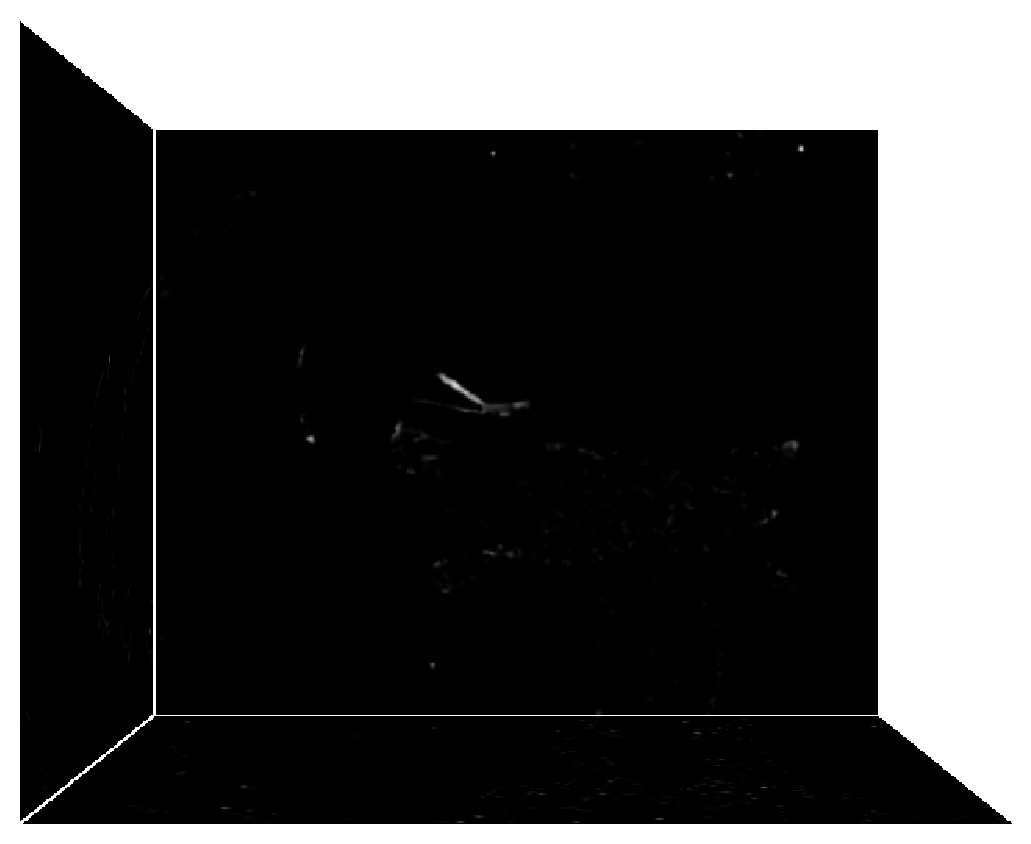
\includegraphics[height=1.5in]{../../Figures/coronary/coronary_enhanced/sigmoid.eps}
\end{figure}
\end{column}
\begin{column}{.5\textwidth}
\onslide<3> \begin{figure}[t]
\centering
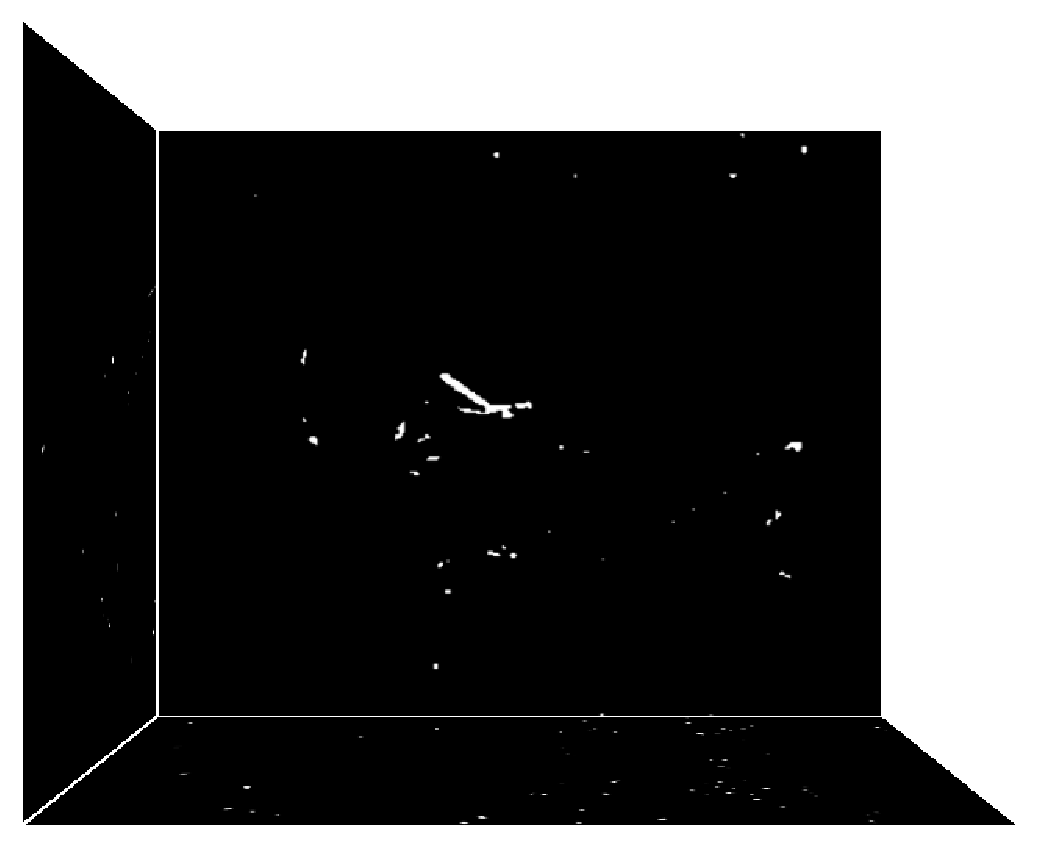
\includegraphics[height=1.5in]{../../Figures/coronary/coronary_enhanced/binary2.eps}
\end{figure}
\end{column}
\end{columns}
\end{frame}

\begin{frame}
\begin{itemize}
  \item \textbf{增强处理后的CURVES演进}:(迭代次数:$50$)
\end{itemize}
\begin{figure}[t]
\centering
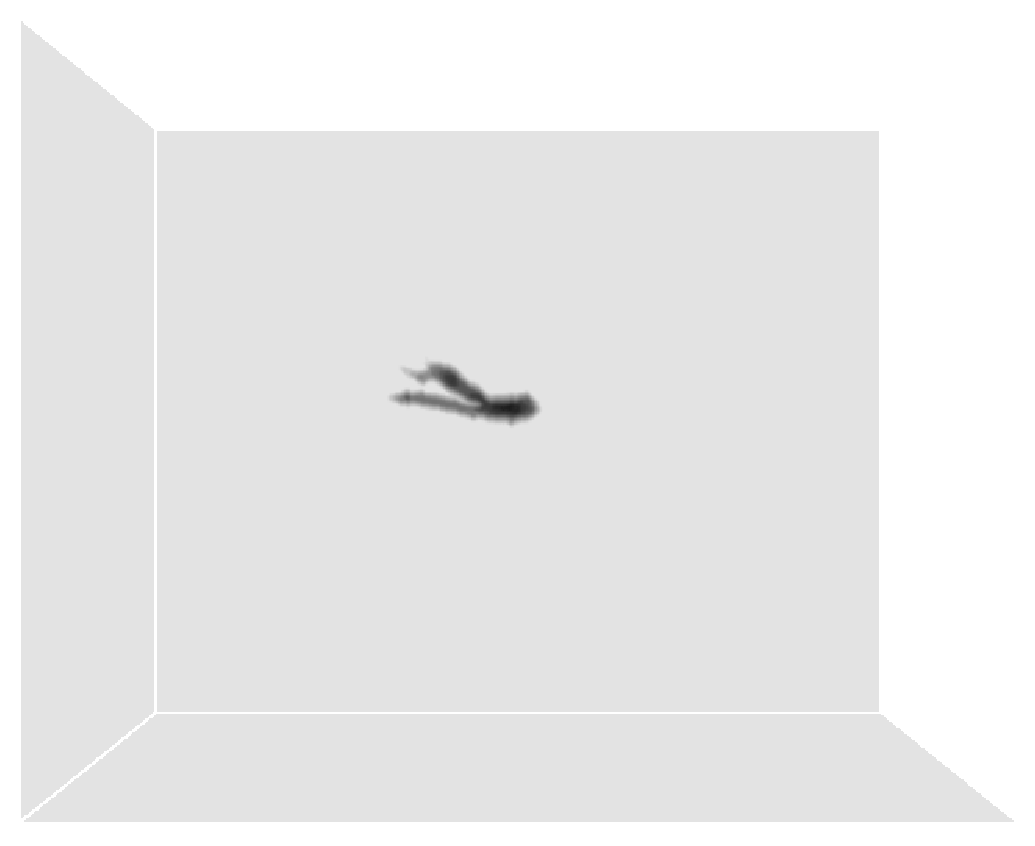
\includegraphics[width=1.5in]{../../Figures/coronary/coronary_enhanced/curves}
% \caption[心脏区域的ROI提取]{心脏区域的ROI提取。}
% \label{fig:coronary_ROI}
\end{figure}
\end{frame}

\begin{frame}
\begin{itemize}
  \item \textbf{冠状动脉模型对比}:
  \begin{enumerate}
    \onslide<1-3> \item 传统CURVES演进结果
    \onslide<3> \item 管状物增强后的CURVES演进结果
  \end{enumerate}
\end{itemize}
\begin{columns}[b,onlytextwidth]
\begin{column}{.5\textwidth}
\onslide<2-3> \begin{figure}[t]
\centering
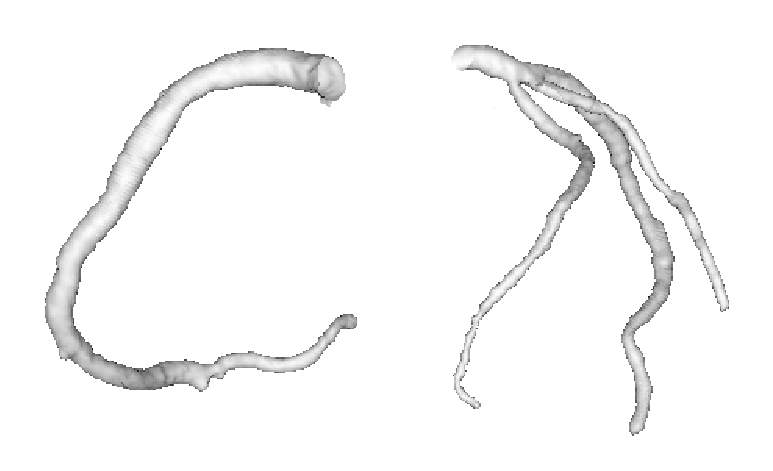
\includegraphics[height=1.2in]{../../Figures/coronary/coronary_enhanced/model_conventional.eps}
\end{figure}
\end{column}
\begin{column}{.5\textwidth}
\onslide<3> \begin{figure}[t]
\centering
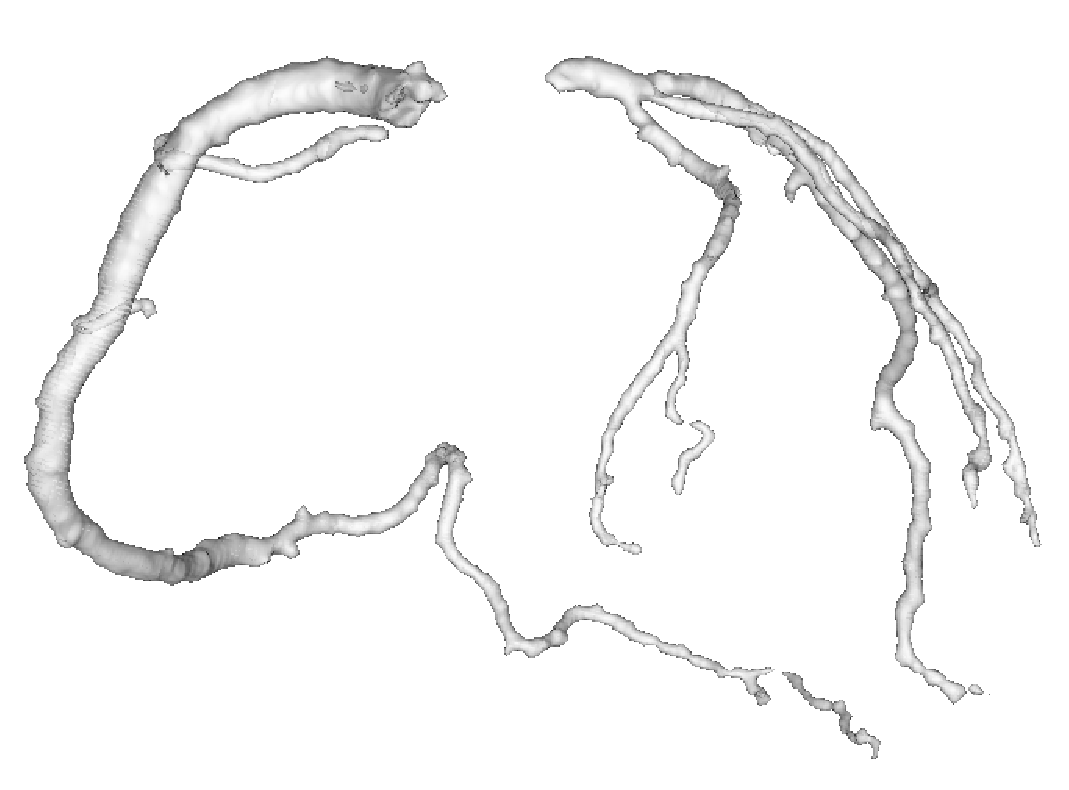
\includegraphics[height=1.2in]{../../Figures/coronary/coronary_enhanced/model_enhanced.eps}
\end{figure}
\end{column}
\end{columns}
\end{frame}

% \begin{frame}

% \end{frame}

% \begin{frame}

% \end{frame} 